\documentclass[12pt,addpoints]{exam}
\usepackage{amsmath}
    \DeclareMathOperator\cis{cis}
\usepackage{amssymb}
\usepackage{tikz}
\usepackage{pgfplots}
    \pgfplotsset{compat=newest}
    
\tikzset{answer/.style={draw,text opacity=0,opacity=0}}
\let\oldprintanswers\printanswers
\def\printanswers{\oldprintanswers\tikzset{answer/.style={text opacity=1,opacity=1,color=red}}}

\usepackage{parskip}

\usepackage{caption}
\DeclareCaptionFormat{empty}{#1}
\renewcommand*\figurename{\sffamily\bfseries Figure}

\setlength{\parindent}{0em}
\setlength{\parskip}{1em}

\usepackage{lastpage}
\footer{}{\iflastpage{\sffamily page~\textbf{\thepage}~of~\textbf{\pageref{LastPage}~--~\textbf{\textit{end of booklet}}}}{\sffamily page~\textbf{\thepage}~of~\textbf{\pageref{LastPage}}}}{\iflastpage{}{\oddeven{\sffamily PLEASE TURN OVER}{}}}

\usepackage{xcolor}
\colorgrids
\definecolor{GridColor}{gray}{0.7}

\makeatletter
\def\fillwithgrid#1{
    \vspace{1ex}
    \fullwidth{
  \begingroup
  \ifhmode
    \par
  \fi
  \hrule height \z@
  \nobreak
  \setlength{\@tempdima}{\gridsize}
  \addtolength{\@tempdima}{\gridlinewidth}
  \setlength{\@tempdimb}{\gridsize}
  \addtolength{\@tempdimb}{-\gridlinewidth}
  \setbox0=\hbox{%
    \rlap{\vrule height \gridsize depth \gridlinewidth width \gridlinewidth}%
    \rlap{\vrule height \gridsize depth -\@tempdimb width \@tempdima}%
    \vrule height 0pt depth \gridlinewidth width \@tempdima
    \llap{\vrule height \gridsize depth \gridlinewidth width \gridlinewidth}%
  }%
  \wd0=\gridsize
  \dp0=0pt
  \setbox1=\hbox to \textwidth{%
    \color@begingroup
    \if@colorgrids
      \color{GridColor}%
    \fi
    \hskip \@totalleftmargin \leaders\copy0\hfil \kern\gridlinewidth
    \color@endgroup
  }
  \cleaders \copy1 \vskip #1 \kern \gridlinewidth \hbox{}%
  \endgroup
  }
      \vspace{-1ex}\droppoints
}

\renewenvironment{solutionorgrid}[1][0pt]%
  {%
    \@insolutiontrue % cancelled by the end of the environment
    \@addpointsfalse % cancelled by the end of the environment
    \ifprintanswers
      \begingroup
      \Solution@Emphasis
      \begin{TheSolution}%
    \else
      \ifcancelspace
        % Do nothing
      \else
        \par
        \penalty 0
        \fillwithgrid{#1}%
      \fi
      \setbox\z@\vbox\bgroup
    \fi
  }{%
    \ifprintanswers
      \end{TheSolution}%
      \endgroup
                \droppoints
    \else
      \egroup
    \fi
  }%
\makeatother


\renewcommand{\d}{\mathrm{d}}

\usepackage{geometry}
    \geometry{
        a4paper,
        margin=2.5cm,
        right=2cm,
        bottom=3cm,
        headheight=14.5pt,
        marginparsep=0mm
    }

\marksnotpoints
\qformat{\textbf{Question~\thequestion}\qquad\qquad(\totalpoints{}~\points)\hfill\vrule depth 3ex width 0pt}
\setlength{\rightpointsmargin}{3cm}
\pointsdroppedatright
\pointformat{(\thepoints)}

\renewcommand{\questionshook}{
    \leftmargin=0pt
    \labelwidth=-\labelsep
}

\usepackage{enumitem}

\renewcommand{\subpartlabel}{(\thesubpart)}

\renewcommand{\solutiontitle}{\noindent\textbf{Solution:}~}
\SolutionEmphasis{\color{red}\sffamily\small}

\usepackage{tkz-euclide}

\newcommand{\blankpage}{
    \pagebreak
    \null
    \vfill
    \begin{center}
        BLANK PAGE
    \end{center}
    \vfill
    \pagebreak
}

\newcommand{\linedpage}{
    \pagebreak
    \begin{framed}
        \lines{26}
    \end{framed}
}

\usepackage{siunitx}

\begin{document}
\sffamily
\begin{coverpages}
{
\renewcommand\labelitemi{$\vcenter{\hbox{\tiny$\bullet$}}$}
\setlist[itemize]{
    itemsep=-1em,
    align=parleft,
    leftmargin=1em,
    labelwidth=0.5em,
    topsep=0em
}
    \begin{minipage}{0.25\linewidth}
        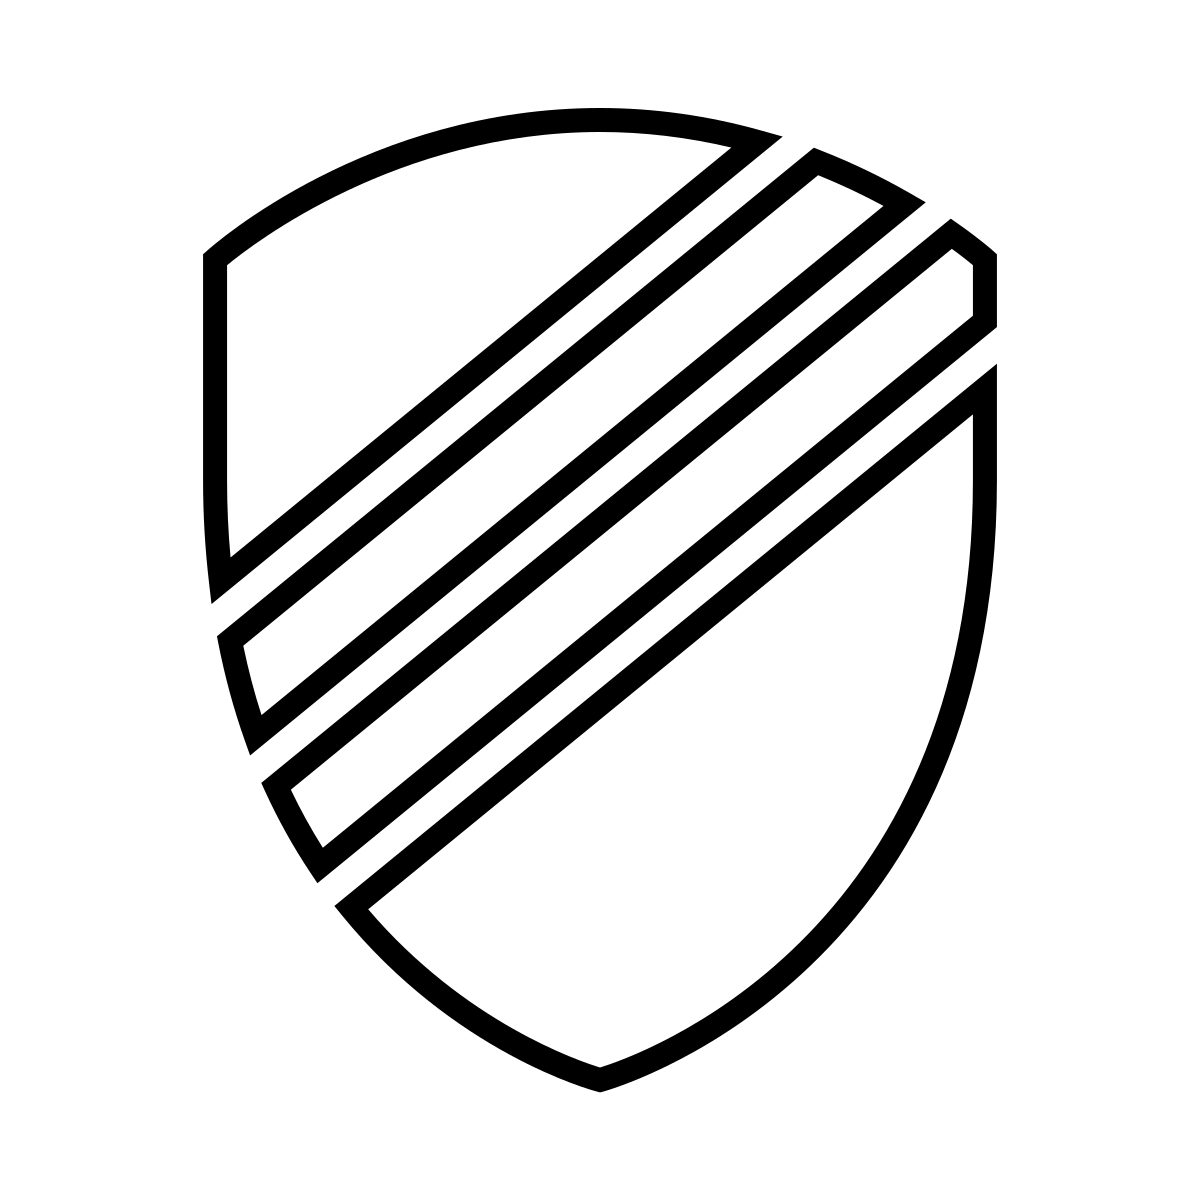
\includegraphics[width=2.9cm]{include/crest.png}
    \end{minipage}
    \begin{minipage}{0.7\linewidth}
        \begin{flushright}
        {\large
            \school\\\vspace{1ex}
            Mathematics Department\\\vspace{1ex}
            \course\\\vspace{1ex}
            \taskyear\\\vspace{1ex}
            \taskname\\\vspace{1ex}
        }
            \end{flushright}
    \end{minipage}
    
    \vspace{1cm}
    \textbf{Question booklet}
    \begin{itemize}
        \item Answer \textbf{\textit{all}} questions
        \item Write your answers in this question booklet
        \item Allow approximately \totaltime minutes
        \item Approved calculators may be used
    \end{itemize}
    \vfill
    \textbf{Examination information}\par
    \textbf{Materials}
    \begin{itemize}
        \item Question booklet
        \item Formula sheet
    \end{itemize}
    \textbf{Instructions}
    \begin{itemize}
        \item Show appropriate working and steps of logic in the question booklets
        \item State all answers correct to three significant figures, unless otherwise instructed
        \item Use black or blue pen
        \item You may use a sharp dark pencil for diagrams
    \end{itemize}
    \textbf{Total time:} \totaltime\\
    \textbf{Total marks:} \numpoints
    \vfill
    Student Name:\ \parbox[b][2em][b]{6cm}{\dotfill}
    \hfill
    Class:\ \parbox[b][2em][b]{5cm}{\dotfill}
}
\end{coverpages}
\addtocounter{page}{1}

%\blankpage
\begin{questions}
\question
\begin{parts}
    \part[1]
    Write $-1+i\sqrt{3}$ in $r\cis\theta$ form.
    \fillwithgrid{2cm}
    \part
    Consider the complex number $z_1=x+iy$, where $x>0$, $y>0$, and $x>y$.\par
    The complex number $z_1$, which lies in the first quadrand of the Argand diagram, is shown in Figure 1.
    \begin{figure}[h]
        \centering
        \begin{tikzpicture}
            \begin{scope}
                \draw[stealth-stealth] (-3,0) -- (3,0) node[right] {$\text{Re}(z)$};
                \draw[stealth-stealth] (0,-2) -- (0,3) node[above] {$\text{Im}(z)$};
                \draw[-stealth] (0,0) -- (2,1) node[right]{$z_1$};
                \draw[dashed] (2,0) -- (2,1) node[midway,right] {$y$};
                \draw (0,0) -- (2,0) node[midway,below]{$x$};
                \draw (0,0) node[below left]{$0$};
            \end{scope}
        \end{tikzpicture}
        \caption[]{}
    \end{figure}
    \begin{subparts}
        \subpart[1]
        Let $z_1=(-1+i\sqrt{3})z_1$.\par
        Using part (a), show that $|z_2|=2|z_1|.$
        \fillwithgrid{4cm}
        \subpart[2]
        On the Argant diagram in Figure 1, draw $z_2$.\par
        \droppoints
    \end{subparts}
    \part[2]
    Use the triangle inequality to show that $|z_1-z_2|<3|z_1|$.
    \fillwithgrid{4cm}
\end{parts}
\end{questions}
\end{document}